\documentclass[11pt,a4paper]{article}
\usepackage[margin=24mm]{geometry}
\usepackage[T1]{fontenc}
\usepackage{lmodern,microtype,graphicx,booktabs,tabularx,longtable,array,amsmath,xcolor}
\usepackage{enumitem,float,caption,fancyhdr,fvextra}
\usepackage[hidelinks]{hyperref}
\definecolor{navy}{HTML}{244E68}
\hypersetup{pdftitle={Tenderworks: Controlled Government Works Estimation},pdfauthor={Tenderworks Project Team}}
\setlength{\parindent}{0pt}
\setlength{\parskip}{6pt}
\setlength{\emergencystretch}{3em}
\renewcommand{\arraystretch}{1.25}
\captionsetup{font=small,labelfont=bf}
\pagestyle{fancy}\fancyhf{}\fancyhead[L]{\small Tenderworks}\fancyhead[R]{\small Technical Report}\fancyfoot[C]{\thepage}
\setlength{\headheight}{14pt}
\newcommand{\fig}[4]{\begin{figure}[H]\centering\includegraphics[width=#3\linewidth,height=.72\textheight,keepaspectratio]{figures/#1.pdf}\caption{#2}\label{#4}\end{figure}}
\newcommand{\pathcode}[1]{\texttt{\detokenize{#1}}}
\begin{document}
\begin{titlepage}
\centering\vspace*{25mm}
{\Huge\bfseries\color{navy} Tenderworks\par}\vspace{8mm}
{\LARGE Controlled, Evidence-Backed Estimation\\for Government Works\par}\vspace{12mm}
{\Large Architecture, Implementation and Empirical Evaluation\par}\vspace{15mm}
{\large Bachelor of Technology Final-Project Technical Report\par}\vspace{7mm}
{17 November 2026\par}
\vfill
\begin{minipage}{.88\textwidth}
\textbf{Demonstrated application.} A scope-limited CPWD PAR 2025 preliminary estimate for a 300\,m$^2$ office in Delhi, using local Ollama inference, document retrieval, deterministic calculations and auditable evidence links.

\textbf{Interpretive boundary.} The implementation demonstrates an integrated estimating workflow. Its drawings are schematic, its benchmark is developer-labelled, and its output requires engineering review before any procurement use.
\end{minipage}
\vspace{18mm}
\end{titlepage}
\pagenumbering{roman}
\section*{Abstract}\addcontentsline{toc}{section}{Abstract}
Government works estimation requires more than a plausible cost response: quantities must correspond to an explicit design basis, rates must satisfy applicability constraints, and calculations must remain reproducible. We develop Tenderworks as a controlled LangGraph workflow with three components: scope and quantity definition, pricing and cost verification, and evidence assurance with document generation. Specialist language-model reviews operate within these components, while software services retain authority over geometry, arithmetic, state transitions and document assembly.

The implemented knowledge layer combines structured rate records, keyword/BM25 document retrieval, immutable source snapshots and controlled web discovery. The demonstrated package transcribes selected CPWD Plinth Area Rates (PAR) 2025 provisions into a narrowly defined preliminary-estimate scenario. The integrated run completed nine Ollama reviews, retrieved twelve excerpts, produced eight downloadable artifacts and calculated a defined-scope total of INR 11,028,540. These observations establish software execution and traceability for the scenario; they do not establish design adequacy.

Evaluation is separated into deterministic tests, isolated agent tasks, checkpoint tests and complete workflows. We verify saved scores against raw outputs before presenting them. In the matched fourteen-case V3 agent experiment, Qwen 2.5 3B passed five cases and Gemma 3 4.3B passed nine. Both executed every task, illustrating the distinction between availability and correctness. Fifty-six automated tests passed in the recorded validation run. We identify engineering-drawing capability as the principal bottleneck: exact arithmetic cannot compensate for incomplete structural, geotechnical or building-services design. The contribution is therefore an auditable estimation architecture and an evaluation methodology that exposes failure, rather than a claim of autonomous tender preparation.

\tableofcontents\clearpage\listoffigures\listoftables\clearpage
\pagenumbering{arabic}
\section{Problem Definition, Objectives and Scope}
Public-works estimates combine technical scope, measurement conventions, schedule applicability and financial treatment. Errors in any of these dependencies can produce a numerically precise but substantively incorrect total. We formulate the task as the conversion of a natural-language brief and explicit project fields into a versioned draft estimate whose quantities, unit rates, adjustments and assumptions can be inspected individually.

The objectives are to (i) preserve an auditable relationship between inputs and costs; (ii) constrain model autonomy within a prescribed process; (iii) expose unsupported scope and missing evidence; (iv) support engineer review and revision; and (v) evaluate interpretation separately from deterministic numerical execution. We do not treat a model confidence score as a substitute for these properties.

\begin{table}[H]\caption{Scope of implementation and validation.}\small
\begin{tabularx}{\linewidth}{lXX}\toprule
Dimension & Implemented capability & Demonstrated boundary \\\midrule
Authority & CPWD, railway and state-PWD routing interfaces & Real-data scenario: CPWD office preliminary estimate \\
Design & Parameterized rectangular layout and stable element IDs & Schematic geometry, not approved engineering drawings \\
Estimation & Structured rates, quantities, adjustments and Decimal arithmetic & Selected PAR composite rates; not a complete detailed DSR BOQ \\
Knowledge & Text retrieval, source snapshots, exact rate lookup & Selectable-text PDFs; no OCR performance established \\
Review & Bounded critique, repair controls, human checkpoints & Critique is advisory; sanction remains external \\
Evaluation & Agent, checkpoint, workflow and tool-level checks & Small developer-labelled corpus; no independent engineering benchmark \\\bottomrule
\end{tabularx}\end{table}

\section{Three-Component Architecture and Responsibility Boundaries}
The orchestration layer is \pathcode{EstimationWorkflow}, implemented as a LangGraph state graph. It owns progression, persistence, repair counters and checkpoint decisions. Local operation uses SQLite state and checkpoint storage; the configuration also supports a PostgreSQL deployment option. Model outputs cannot independently change the graph, approve estimates, modify official rates or execute arbitrary programs.

Figure~\ref{fig:architecture} presents the three-component architecture. The editable source is retained as a Mermaid file; its rendered vector output is incorporated into this LaTeX report. Retrieval is performed through the shared application gateway and supplied as bounded context to model calls. The current Ollama adapter is not a freely acting tool-selection agent.
\begin{figure}[p]\centering
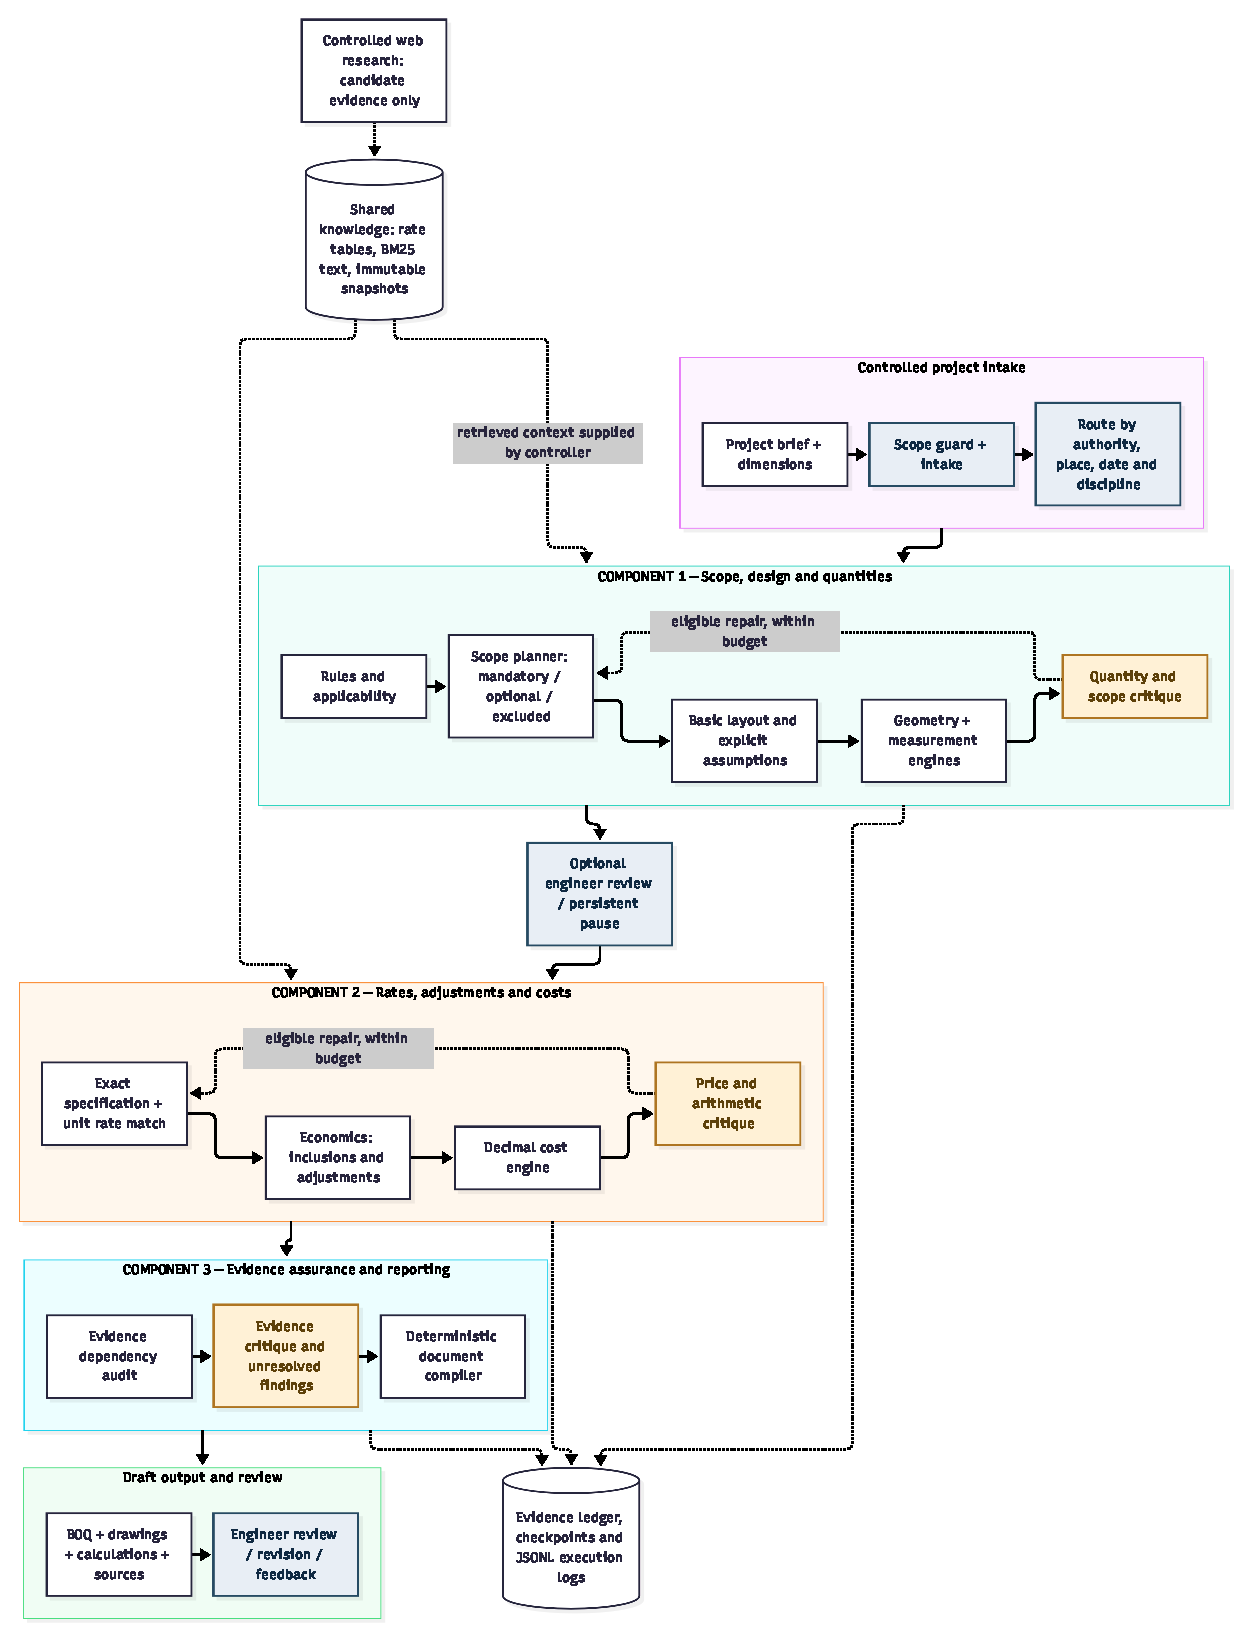
\includegraphics[width=\linewidth,height=.87\textheight,keepaspectratio]{figures/architecture.pdf}
\caption{Detailed three-component architecture. Solid arrows indicate workflow progression; dashed connections indicate repair or shared evidence dependencies.}\label{fig:architecture}
\end{figure}

\subsection{Component 1: Scope, Design and Quantities}
Intake extracts supported facts, while explicit form fields provide a structured project basis. Routing considers authority, location, date and work category. Rules and scope roles identify applicable provisions and classify items as required, optional or excluded. A parameterized design model supplies basic geometry, after which deterministic measurement recipes generate quantities and worksheets. Scope and quantity critique checks omissions, duplication, units and links to design elements. The output is a versioned quantity baseline with assumptions and findings.

\subsection{Component 2: Rates, Adjustments and Cost Verification}
Rate selection uses structured records with compatible specifications and units. Economics review identifies inclusions and applicable adjustments, while the cost engine computes amounts using Decimal arithmetic. Price critique examines inconsistencies and potential double counting. Scheduled versus non-scheduled classification controls the rate basis; fixed, quantity-dependent and time-dependent classifications describe cost behaviour. These are separate dimensions.

\subsection{Component 3: Evidence Assurance and Reporting}
The evidence audit traverses dependencies among sources, quantities, rates and calculations. The report compiler produces spreadsheets, narrative estimates and drawings from persisted artifacts. An incomplete rate or quantity remains visible; a required unresolved item cannot silently become a zero-cost item. Final output status distinguishes a draft from an incomplete result and from a separately recorded engineering review decision.

\begin{table}[H]\caption{Responsibilities of agents and deterministic services.}\small
\begin{tabularx}{\linewidth}{p{.23\linewidth}XX}\toprule
Responsibility & Model contribution & Software authority \\\midrule
Intake and routing & Structured fact extraction & Schema, explicit fields and package filters \\
Rules and scope & Evidence-grounded review and omissions & Applicability checks and component templates \\
Design and quantities & Review of assumptions and discrepancies & Geometry, unit handling and measurement recipes \\
Rates and economics & Review of matches, inclusions and adjustments & Rate selection constraints and executable inputs \\
Verification & Bounded concerns and cited excerpts & Arithmetic, evidence-ID validity and status rules \\
Evidence and reporting & Advisory critique of evidence gaps & Dependency checks, exports and revision history \\\bottomrule
\end{tabularx}\end{table}

\section{Control Strategy, Critique and Human Review}
We initially explored greater agent autonomy and subsequently adopted explicit checkpoints to align the implementation with a prescribed estimating process. We also introduced critique roles after observing deficiencies in early outputs. These are qualitative development observations. No controlled ablation was conducted, so the experiments in this report cannot quantify a causal benefit from adding critics or reducing autonomy.

The implemented control strategy uses bounded, targeted correction rather than unconstrained debate. Eligible scope omissions or duplication findings can trigger scope repair; arithmetic mismatch can trigger price repair. The configured limit ranges from zero to five attempts per supported checkpoint, with a default of two. An authorized skip request prevents further retries after the current operation; it does not interrupt an in-flight model call or erase unresolved findings. Figure~\ref{fig:control} specifies this decision logic.
\fig{control}{Checkpoint validation, bounded correction and progression. Exhausting the budget changes control flow, not the truth of unresolved findings.}{1}{fig:control}

Optional engineer review pauses after the first checkpoint. Persistent state permits subsequent continuation. Final review is a distinct action; neither a successful critique call nor an exhausted retry budget constitutes approval. Feedback can create a new project revision or a proposed regression case. It does not overwrite official rates or automatically train the model.

A recorded regression test forces an unresolved component finding, exhausts two repair cycles and verifies that reporting is still reached with the blocker and incomplete total retained. This establishes the behaviour of the control policy for that test; it does not demonstrate that additional iterations improve estimate accuracy. A future ablation should hold projects and model versions constant while varying critique and repair budgets.

\section{Data Corpus, Provenance and Ingestion Method}
The active corpus comprises the CPWD PAR 2025 PDF and a structured preliminary-office domain package. The package is deliberately classified for demonstration use: official numerical transcriptions coexist with assumed geometry and service selections. The official origin of a rate does not validate the assumed engineering design.

\begin{table}[H]\caption{Document corpus and ingestion status. Byte counts are checked against the saved download manifest.}\small
\begin{tabularx}{\linewidth}{Xrrp{.24\linewidth}}\toprule
Document & Bytes & Indexed & Role \\\midrule
CPWD PAR 2025 & 5,341,115 & Yes & Preliminary area rates and provisions \\
Railway Board CPWD adoption notice (2025) & 189,422 & No & Archived authority context \\
Maharashtra PWD SSR 2022--23 & 8,296,605 & No & Archived expansion material \\
DAR Vol. I, updated December 2021 & --- & No & Existing user-supplied archive; not independently acquired in this study \\\bottomrule
\end{tabularx}\end{table}

Each downloaded snapshot has a recorded URL, acquisition metadata, byte count and SHA-256 digest. Before preparing this report, we recomputed the hashes and sizes of all three downloaded documents and confirmed agreement with the manifest. Railway and state-PWD files are retained outside the scanned directory and therefore do not contribute to the demonstrated real-data RAG coverage.

Ingestion fingerprints file content and associated metadata. New or changed sources are extracted and indexed; unchanged fingerprints are skipped. This is an idempotence mechanism, not evidence that every extracted value is semantically correct. Selectable PDF text is read using pypdf, partitioned into retrievable chunks and associated with immutable source snapshots. The current path does not perform OCR. Scanned schedules, complex tables and footnote-dependent rates require additional preprocessing and validation.

The measured retrieval configuration uses keyword/BM25 search. Optional embeddings exist in the implementation, but no vector-retrieval performance claim is made. Structured numeric records are kept distinct from descriptive retrieval. Domain packages bind rate records, applicability conditions, measurement recipes, design templates and validation policies to an explicit version.

\subsection{Retrieval Evaluation and Its Interpretation}
The saved retrieval test contains one expected source and textual match. It achieved recall@5 of 1.00 and reciprocal rank of 1.00, meaning the expected match was returned first in that test. This is a functional retrieval check, not a corpus-wide estimate of recall. The integrated CPWD run retrieved twelve excerpts, which measures retrieval activity rather than relevance precision. More defensible retrieval evaluation requires multiple questions, engineer-labelled relevant passages, distractor documents, amendments and obsolete editions.

\section{Web Evidence, Guardrails and Auditability}
The application offers two web modes. The key-free official mode searches a restricted publication index for the supported PAR document; it is not a general-purpose search engine. Brave mode supports wider discovery when credentials are configured. Requests enforce HTTPS/domain restrictions, public-address checks, redirect validation, bounded payloads and timeouts. Successful candidates are cached per tenant and query for twenty-four hours.

Web content enters as candidate evidence. RAG content is also subject to provenance and applicability checks; local storage alone does not confer authority. Only supported structured rate records participate in numerical calculation. In the final integrated run, web discovery reused one cached official candidate, reported no retrieval error and retained the candidate-review status. This supports the cache and disclosure path, not independent validation of the candidate's suitability.

\begin{table}[H]\caption{Guardrail criteria and residual limitations.}\small
\begin{tabularx}{\linewidth}{p{.22\linewidth}XX}\toprule
Boundary & Implemented criterion & Remaining concern \\\midrule
Task scope & Reject obvious unrelated requests before model invocation & Heuristic intent checks may miss ambiguous wording \\
Model output & JSON schema, bounded fields and cited evidence checks & Valid syntax does not imply correct meaning \\
Rate authority & Applicable structured records and unit/specification checks & Coverage depends on validated domain packages \\
Web input & Restricted retrieval and candidate trust labels & Network defence and document semantics require further hardening \\
Calculation & Restricted arithmetic expressions and Decimal values & Correct computation can use incorrect engineering assumptions \\
Review & Explicit findings and separate human decisions & Reviewer competence remains outside software validation \\\bottomrule
\end{tabularx}\end{table}

The evidence ledger is a dependency register, not merely a list of URLs. A BOQ amount links to its quantity calculation and effective rate; those records link to design inputs, documents, adjustments and assumptions. Structural coverage therefore indicates the presence of required links, not that their content is semantically entailed or professionally adequate.

Tenant- and revision-separated JSONL logs retain node inputs and outputs, model responses, failures, roles, duration and usage metadata. The logs record observable outputs rather than hidden reasoning. Optional redaction replaces text bodies with hashes. Retention is enforced through an explicit purge command. Local application logs are not automatically uploaded to LangSmith; benchmark publication is opt-in. These controls make failures inspectable while preserving a boundary between operational data and curated evaluation data.

\section{Engineering Drawings, Quantity Validity and the CPWD Case Study}
\subsection{Engineering Drawings as the Principal Bottleneck}
The geometry engine constructs rectangular layouts with stable identifiers for walls, rooms, slabs and openings. The same geometric representation supports SVG, PDF and DXF export. This consistency is useful for traceability, but geometric consistency must not be confused with engineering adequacy. The engine does not perform geotechnical interpretation, foundation selection, structural analysis, reinforcement detailing, services sizing, clash detection or statutory design verification.

\textbf{The engineering-drawing subsystem is the principal bottleneck in extending this prototype to detailed government tender estimation.} A convincing drawing can still omit the information required to measure reinforcement, foundations or mechanical and electrical installations. RAG can retrieve specifications, and a model can identify concerns, but neither establishes the physical adequacy of an unanalysed design. Additional critique cycles cannot compensate for missing design calculations.
\fig{geometry}{Propagation of design limitations into quantity and cost estimation. A shared geometry model improves traceability but does not supply missing engineering design.}{1}{fig:geometry}

For an item amount $A_i=q_i r_i$, first-order sensitivity is
\begin{equation}
\Delta A_i \approx r_i\Delta q_i + q_i\Delta r_i.
\end{equation}
Thus, even with an exact unit rate, quantity error propagates directly into cost. This relationship explains why pricing accuracy alone cannot establish estimate accuracy. In the current PAR case, the dominant shell quantity is floor area; the demonstration largely bypasses the detailed component take-off needed for a DSR tender BOQ. Its successful total therefore provides especially limited evidence about the quality of the drawing engine.

\begin{table}[H]\caption{Engineering capability gap and proposed validation evidence.}\small
\begin{tabularx}{\linewidth}{p{.23\linewidth}XX}\toprule
Engineering task & Current basis & Evidence required for extension \\\midrule
Architectural layout & Rectangular template and assumed dimensions & Approved-layout comparisons and dimensional constraints \\
Foundation/structure & No structural adequacy calculation & Soil inputs, load analysis and reviewed member design \\
Reinforcement & Allowances or unresolved detailed quantities & Bar-bending schedules and measured take-off comparison \\
Building services & Scenario selections and percentage provisions & Load/capacity sizing and coordinated service drawings \\
Quantity validation & Formula and unit consistency & Independent quantity surveyor measurements \\\bottomrule
\end{tabularx}\end{table}

Future work should first integrate engineer-reviewed design templates and measurement rules, then validate quantity error by component against independently prepared drawings. Suitable measures include dimensional deviation, omission rate, per-component quantity error and cost-weighted error. These are proposed measures; no such engineering-design benchmark has yet been executed.

\subsection{Scenario Definition and Source-Based Arithmetic}
The demonstrated brief specifies a 300\,m$^2$, single-storey office in Delhi, a 3.60\,m storey height and a 2025 rate basis. The package selects an office shell, assumed downcomer and manual alarm provisions, internal water supply and internal electrical services. Fire-system selection is a scenario assumption, not a compliance determination. Gross floor area is provisionally used as plinth area and requires engineering measurement review.

\begin{table}[H]\caption{CPWD preliminary-estimate calculation. Page numbers denote PDF page positions.}\small
\begin{tabularx}{\linewidth}{Xllr}\toprule
Item and source & Basis & Calculation & Amount (INR) \\\midrule
Office shell: 1.1.1, p.13 & INR 30,920/m$^2$ & $300\times30{,}920$ & 9,276,000 \\
Downcomer: 1.5.1, p.14 & INR 460/m$^2$ & $300\times460$ & 138,000 \\
Manual alarm: 1.6.1, p.14 & INR 280/m$^2$ & $300\times280$ & 84,000 \\
Internal water: 2.1, p.14 & 4\% of shell & $0.04\times9{,}276{,}000$ & 371,040 \\
Internal electricity: 2.3, p.15 & 12.5\% of shell & $0.125\times9{,}276{,}000$ & 1,159,500 \\\midrule
\multicolumn{3}{l}{Defined-scope preliminary total} & \textbf{11,028,540} \\\bottomrule
\end{tabularx}\end{table}
\fig{cost_composition}{Cost composition of the defined CPWD scope. The shell dominates the total; this does not establish that omitted works are immaterial.}{.95}{fig:cost}

The shell contributes approximately 84.1\% of the defined total. Accordingly, area interpretation and applicability of the shell rate dominate this scenario. External development and connections, land, lifts, HVAC, solar, consultancy, TPQA, local approvals and escalation are excluded. No additional tax treatment is inferred. The figure is a 2025-basis preliminary estimate of the specified scope, not a current market quotation or sanctioned budget.

\subsection{Integrated Execution Evidence}
The persisted demonstration revision is \pathcode{8690eaa8-fe78-49f8-9770-620f440f110e}. It reached draft status with nine successful Ollama specialist traces and no model-unavailable finding. All eight exported artifacts returned HTTP 200 during the recorded download checks.
\begin{table}[H]\caption{Integrated CPWD execution observations and their meaning.}\small
\begin{tabularx}{\linewidth}{l r X}\toprule
Observation & Value & Interpretation \\\midrule
Ollama specialist traces & 9 & Live reviews completed; their correctness is evaluated separately \\
Model-unavailable findings & 0 & No recorded provider failure in this run \\
Retrieved excerpts & 12 & Retrieval participated in the workflow \\
Structural evidence coverage & 1.00 & Required priced-row evidence links were present \\
Successful artifact downloads & 8/8 & Export endpoints served their outputs \\
Defined-scope total (INR) & 11,028,540 & Matches the stated deterministic calculation \\\bottomrule
\end{tabularx}\end{table}
The artifacts comprise BOQ XLSX, estimate PDF/DOCX/JSON, concept SVG/PDF/DXF and a ZIP bundle. Successful download does not assess graphical design quality or engineering completeness.

\section{Evaluation Methodology and Data Verification}
\subsection{Layered Experimental Design}
We separate four levels of evaluation to localize failure. Tool-level tests establish numerical and state invariants. Isolated agent tests measure interpretation and evidence-grounded responses. Checkpoint tests provide deterministic upstream fixtures to isolate selected responsibilities. Complete workflows test progression, expected abstention and final outputs. LangSmith's evaluation SDK executes examples and records outputs and evaluator scores locally; hosted upload was not exercised because credentials were not supplied.

The V3 dataset contains twenty-seven cases: fourteen isolated agent cases and thirteen cases across other layers. The matched model comparison uses the same fourteen agent cases: five intake examples, eight specialist defect examples and one clean critic example. Cases named ``unseen'' are additional development diagnostics; their names do not establish independent held-out evaluation.

\subsection{Verification of Saved Results}
Before report generation, we recomputed every stored per-case score using the evaluator and checked summary counts, macro means, latency medians and discrete p95 values. We also checked the dataset, package and source-tree hashes for the matched V3 pair and the local PDF snapshots against their manifests. The audit is saved in \pathcode{report/evaluation_audit.json}. This verifies internal reproducibility of the reported numbers, not the correctness of developer-authored labels or the evaluator's construct validity.

The principal comparison uses \pathcode{v3-qwen-agents} and \pathcode{v3-gemma-agents}. Other timestamped runs and earlier V1/V2 experiments are retained but are not pooled to enlarge the primary sample. Earlier versions differ in prompts, output budgets and, in V3, one corrected intake label and two added cases. Their aggregate scores cannot be interpreted as a controlled before/after improvement.

\subsection{Metric Definitions and Limitations}
\begin{table}[H]\caption{Operational definitions of evaluation metrics.}\small
\begin{tabularx}{\linewidth}{p{.22\linewidth}XX}\toprule
Metric & Computation & Interpretive limitation \\\midrule
Field precision / recall & Correct exact field-value pairs divided by predicted / expected fields; macro-averaged per case & Penalizes contract mismatch; not broad language understanding \\
Quote grounding & All returned fact quotes occur in the input, with nonempty quote text & Empty fact sets can satisfy the quote predicate vacuously \\
Citation grounding & Fraction of concerns with a valid evidence ID and exact source substring & Does not prove that the quote supports the concern \\
Defect recall proxy & Expected evidence IDs recovered among grounded concerns & Evidence identity is a proxy for semantic defect detection \\
No extra grounded ID & No detected grounded evidence ID lies outside the expected set & Ungrounded concerns are not counted by this predicate \\
Strict case pass & All applicable case assertions succeed & Stronger than schema validity; still limited by labels and proxies \\
Arithmetic exactness & Priced amounts equal rounded quantity times rate & Can be vacuously true when no priced rows exist \\
Evidence coverage & Required evidence links on priced rows are present & Structural connectivity, not semantic truth \\
Model availability & Non-unavailable model calls divided by model calls & Offline runs have a default value; not live inference evidence \\
Recall@k / reciprocal rank & Expected source match in top k / inverse first-match rank & Current retrieval result covers one query only \\\bottomrule
\end{tabularx}\end{table}
For extraction, if $c$ denotes correctly matched fields, $p$ predicted fields and $g$ expected fields, precision is $c/p$ and recall is $c/g$, with explicit empty-set conventions in the evaluator. Reported values are macro means over cases where the metric applies. We do not mix five-case extraction denominators with nine-case critique denominators.

\section{Agent Benchmark Results and Interpretation}
\subsection{Controlled Comparison Protocol}
The models are Qwen 2.5 3B (recorded parameter size 3.1B) and the installed Gemma 3 model (4.3B), both Q4\_K\_M quantizations. Tests ran sequentially on an Apple M1 system with 8\,GB memory, Python 3.12.4, temperature zero and one repetition per case. The V3 prompt identifier is \pathcode{2026-11-17-bounded-review-v3}. Matched hashes confirm identical benchmark source, dataset and package within this comparison. Benchmark inference used an 8,192-token context and 900-token output budget; the integrated local demo used a 4,096-token context and a longer timeout. These are distinct experiments.

\begin{table}[H]\caption{V3 agent scores recomputed from raw outputs. Case counts identify the denominator of each macro mean.}\small\begin{tabularx}{\linewidth}{Xrrr}
\toprule
Metric & Cases & Qwen & Gemma \\
\midrule
Strict case pass & 14 & 0.3571 & 0.6429 \\
Field precision & 5 & 0.6143 & 0.8000 \\
Field recall & 5 & 0.5000 & 0.8000 \\
Exact-quote grounding & 5 & 0.8000 & 0.6000 \\
Citation grounding & 9 & 0.6111 & 0.8889 \\
Defect recall proxy & 9 & 0.5556 & 0.7778 \\
No extra grounded evidence ID & 9 & 0.8889 & 0.8889 \\
\bottomrule
\end{tabularx}
\end{table}
\fig{agent_metrics}{Matched V3 agent metrics. Execution succeeded in all fourteen cases for each model, but strict pass rates were substantially lower.}{1}{fig:metrics}

Qwen passed 5/14 cases (35.7\%) and Gemma passed 9/14 (64.3\%). The observed difference is 28.6 percentage points on this dataset. Descriptive Wilson intervals for the case pass proportions are approximately 16.3--61.2\% and 38.8--83.7\%, respectively. Cases are heterogeneous, developer-authored and not sampled independently from a project population; these intervals do not justify a general model-ranking claim.

\subsection{Extraction and Grounding Failures}
Gemma achieved macro field precision and recall of 0.80, compared with Qwen's 0.6143 precision and 0.50 recall. However, exact-quote grounding was 0.60 for Gemma and 0.80 for Qwen. This illustrates a trade-off within the observed outputs: stronger field matching did not automatically yield better supporting quotations. Qwen passed none of the five intake cases under the combined strict criterion; Gemma passed two. Therefore, neither model should be treated as a reliable unsupervised intake authority on the basis of these tests.

Critique citation-grounding scores were 0.6111 for Qwen and 0.8889 for Gemma. Defect-recall proxies were 0.5556 and 0.7778. These indicate better evidence-ID/substring compliance by Gemma in this experiment, not proof of more accurate engineering reasoning. Both models scored 0.8889 on the ``no extra grounded ID'' predicate, but both failed the clean critic case. The aggregate predicate must therefore not be described as a general false-positive rate: it considers grounded IDs only and does not measure all unsupported assertions.
\fig{case_matrix}{Per-case strict outcomes. The clean critic case fails for both models; evidence-audit behaviour differs from the broader aggregate ranking.}{1}{fig:cases}
\begin{table}[H]\caption{Detailed case outcomes for the matched V3 comparison.}\small\begin{tabularx}{\linewidth}{Xll}
\toprule
Case & Qwen & Gemma \\
\midrule
intake-0 & Fail & Fail \\
intake-1 & Fail & Pass \\
intake-2 & Fail & Fail \\
scope-defect & Pass & Pass \\
design-defect & Pass & Pass \\
rules-defect & Fail & Pass \\
quantity\_verifier-defect & Pass & Pass \\
rate\_estimator-defect & Fail & Pass \\
economics-defect & Pass & Pass \\
pricing\_verifier-defect & Fail & Pass \\
evidence\_audit-defect & Pass & Fail \\
critic-clean & Fail & Fail \\
intake-unseen-railway & Fail & Pass \\
intake-unseen-office & Fail & Fail \\
\bottomrule
\end{tabularx}
\end{table}

The case-level evidence shows why a single overall score is insufficient. Qwen passed the evidence-audit defect case while Gemma failed it, despite Gemma's higher overall pass rate. Both models passed the scope, design, quantity-verifier and economics defect examples. These are isolated controlled examples, not validation of each role across realistic project variation.

\subsection{Latency and Resource Implications}
\begin{table}[H]\caption{Target latency in the matched experiment. The recorded p95 is the discrete order statistic selected by the harness.}\small\begin{tabularx}{\linewidth}{Xrrr}
\toprule
Model & p50 (s) & p95 (s) & Execution \\
\midrule
qwen2.5:3b & 13.17 & 16.73 & 14/14 \\
gemma3:latest & 10.02 & 14.74 & 14/14 \\
\bottomrule
\end{tabularx}
\end{table}
\fig{latency}{Per-case target latency. Prompt composition and task type affect response time, so aggregate medians do not represent full-workflow latency.}{.98}{fig:latency}
Gemma's median target latency was 10.02 seconds, compared with 13.17 seconds for Qwen. At fourteen observations, the harness's p95 selection is the largest observed latency, 14.74 seconds for Gemma and 16.73 seconds for Qwen. Warm/cold loading and shared-memory conditions were not controlled as a dedicated systems experiment. The results support a local responsiveness comparison under the recorded run, not a hardware-independent throughput claim.

\section{Checkpoint Validation, Workflow Reliability and Technical Findings}
\subsection{Deterministic and Workflow Results}
\begin{table}[H]\caption{Recorded non-agent verification results. These tests answer different questions and are not pooled into one accuracy score.}\small
\begin{tabularx}{\linewidth}{Xrl}\toprule
Verification & Result & Evidence artifact \\\midrule
Automated regression tests & 56 passed & validation.json \\
Isolated deterministic checkpoint cases & 4/4 & offline-checkpoints \\
V3 deterministic complete workflows & 3/3 & v3-offline-workflow \\
Expected-source retrieval query & 1/1 & offline-retrieval \\
Integrated CPWD live model calls & 9/9 available & final-demo-check.json \\
Integrated export downloads & 8/8 & final-demo-check.json \\\bottomrule
\end{tabularx}\end{table}
The checkpoint suite covers CP1, CP2, CP3 and a corrupted-evidence CP3 case. The last case passes when the system correctly identifies the evidence defect, rather than accepting an invalid estimate. The three V3 workflow cases cover the CPWD scenario, an off-topic request and an unsupported project. A pass therefore includes correct refusal or incompleteness, not only a completed priced estimate.

These observations support deterministic calculation, controlled progression and expected failure handling in the tested cases. They do not establish comprehensive engineering correctness. In particular, offline runs cannot demonstrate model availability, and arithmetic exactness on an abstention with no priced rows is not evidence of pricing accuracy. We consequently avoid interpreting the mixed checkpoint average of evidence coverage as a project-quality statistic.

\subsection{Technical Problems and Implemented Responses}
\begin{table}[H]\caption{Substantive technical findings and remaining limitations.}\small
\begin{tabularx}{\linewidth}{p{.24\linewidth}XX}\toprule
Problem & Implemented response & Residual limitation \\\midrule
Searchable prose is not executable rate knowledge & Versioned structured PAR package with source locators & Detailed DSR coverage requires reviewed mappings \\
Design assumptions dominate quantity validity & Shared geometry IDs and explicit quantity basis & Structural and services design remain absent \\
Scope exclusions misinterpreted as inclusions & Clause-level exclusion handling and regression case & Complex mixed-language scope remains difficult \\
Numeric strings violate downstream contracts & Separator normalization and explicit numeric schema instructions & Model extraction errors persist in V3 results \\
Long model outputs exceed practical budgets & Bounded review fields, output budget and timeout controls & Limited context can omit relevant evidence \\
Open-ended correction lacks termination guarantees & Bounded targeted repairs and audited skip control & Additional iterations cannot resolve missing design data \\
Successful execution obscures incorrect answers & Separate availability, grounding and strict reference metrics & Semantic adjudication remains necessary \\
Insufficient observability for diagnosis & Structured model/node logs and retained raw evaluation outputs & Operational privacy and retention require deployment policy \\\bottomrule
\end{tabularx}\end{table}

The benchmark demonstrates a central systems distinction: a robust workflow can calculate an auditable draft while its advisory models remain unreliable on isolated interpretation tasks. Numerical authority, source applicability and human review should therefore remain outside unrestricted model control. Conversely, deterministic calculations alone cannot guarantee the adequacy of their engineering inputs.

\section{Limitations, Future Work and Conclusions}
\subsection{Threats to Validity}
The benchmark is small, developer-labelled and used during development. No independent engineer panel adjudicated outputs, no project-family split establishes generalization, and no multi-repetition stability study was completed. Evidence-ID and exact-substring metrics do not test semantic entailment. Model comparison is limited to two quantized local models on one machine. The CPWD scenario uses a composite PAR method and assumed service selections; it cannot validate detailed structural take-off or all-authority routing with real data.

\subsection{Prioritized Development Programme}
The first priority is engineering design and quantity validation. We propose integrating reviewed architectural and structural inputs, explicit measurement standards and independent quantity-survey benchmarks. A useful release criterion would require accepted tolerances for major component quantities and documented treatment of unresolved design conditions, rather than a visually convincing drawing alone.

The second priority is a larger independently labelled evaluation corpus with source amendments, conflicting editions, adversarial instructions, multilingual briefs and unsupported cases. Repeated runs, engineer adjudication, semantic citation assessment and controlled critique-loop ablations should follow. The third priority is operational hardening: production authentication, network isolation, load tests, backup/restore validation, monitoring and reviewed data-retention procedures.

\subsection{Conclusion}
We have implemented and demonstrated an auditable three-component workflow that combines constrained language-model review with deterministic estimation services. The scoped CPWD example completes retrieval, model review, calculation and export, while the evaluation framework exposes substantial interpretation and grounding failures. The architecture is therefore a foundation for engineer-supervised estimation, not evidence of autonomous government tender readiness. Further progress depends most strongly on validated engineering drawings and quantities, followed by broader source coverage and independently adjudicated evaluation.

\section{Experimental Reproducibility and Project Organisation}
\subsection{Repository Structure}
The following ASCII tree is a simplified view of the implemented repository. Runtime directories are shown for operational clarity; they are excluded from version control.
\begin{Verbatim}[fontsize=\small]
TendorWorks/
|-- src/tender/
|   |-- workflow.py          # LangGraph controller
|   |-- agents.py            # Specialist responsibilities
|   |-- providers.py         # Model adapters and schemas
|   |-- engines.py           # Geometry and calculations
|   |-- ingestion.py         # Incremental source ingestion
|   |-- knowledge.py         # Retrieval and rate access
|   |-- research.py          # Controlled web retrieval
|   |-- guardrails.py        # Scope screening
|   |-- observability.py     # Structured execution logs
|   |-- benchmarks.py        # Layered evaluation harness
|   |-- exports.py           # Estimate and drawing outputs
|   `-- static/              # Browser interface
|-- database/cpwd/           # Active PDF and domain package
|-- reference_documents/     # Archived, non-indexed documents
|-- examples/                # Reproducible project briefs
|-- eval/
|   |-- datasets/            # Versioned labelled examples
|   `-- results/             # Raw runs and summary metrics
|-- tests/                   # Deterministic regression tests
|-- scripts/                 # Data, demo and report utilities
|-- report/
|   |-- FINAL_REPORT.tex     # Canonical academic report
|   |-- FINAL_REPORT.pdf     # Compiled LaTeX output
|   |-- diagrams/            # Editable Mermaid sources
|   |-- figures/             # Vector figures and PNG previews
|   `-- evaluation_audit.json
|-- docs/                    # Guardrail and provenance detail
|-- var/                     # Local state, snapshots and logs
`-- outputs/                 # Generated runtime artifacts
\end{Verbatim}

\subsection{Execution Protocol}
The application environment is resolved from the repository lockfile. Ollama must be running with the selected model available. The exact CPWD brief is stored in \pathcode{examples/cpwd-office-demo.json}; changing its date, authority, scope or geometry can legitimately change applicability and results.
\begin{Verbatim}[fontsize=\small,breaklines=true]
uv sync --frozen
uv run tender ingest
uv run python scripts/run_demo.py
uv run tender serve --port 8000
\end{Verbatim}
The local environment uses the Ollama provider and the existing example configuration. The documented offline mode is a distinct deterministic verification path, not a replacement for live-model evaluation. Review of the resulting revision should include findings, assumptions, source links and excluded scope before examining the total.

\subsection{Evaluation and Report Regeneration}
The matched comparison is reproduced using the versioned fourteen-case dataset and separate result directories. Actual future outputs may differ even with nominally deterministic inference.
\begin{Verbatim}[fontsize=\small,breaklines=true]
uv run python -m tender.benchmarks --dataset eval/datasets/model-comparison-v3.json --model qwen2.5:3b --output eval/results/reproduction-qwen
uv run python -m tender.benchmarks --dataset eval/datasets/model-comparison-v3.json --model gemma3:latest --output eval/results/reproduction-gemma
uv run pytest -q
\end{Verbatim}
The report build verifies saved measurements, generates Matplotlib figures and tables, renders Mermaid diagrams and compiles this LaTeX source using Tectonic. Detailed build prerequisites and commands are recorded in \pathcode{report/BUILD.md}. The canonical report is the LaTeX/PDF pair; the earlier Word report is a historical export and is not the revised submission document.

\subsection{Data and Software Documentation}
CPWD PAR 2025 is preserved at \pathcode{database/cpwd/PAR_2025.pdf}, with the original publication URL and file fingerprint in \pathcode{reference_documents/download_manifest.json}. The structured scenario and page locators are described in \pathcode{docs/DATA_SOURCES.md}. Guardrail criteria are recorded in \pathcode{docs/GUARDRAILS.md}, and evaluation details in \pathcode{evals_final.md}.

The architecture uses LangGraph for stateful orchestration and the LangSmith SDK for local experiments. The report's numerical claims are linked to repository artifacts rather than undocumented aggregate impressions. Full raw outputs are retained for independent examination of scoring assumptions and failure cases.
\end{document}
